\begin{figure*}
    \centering
    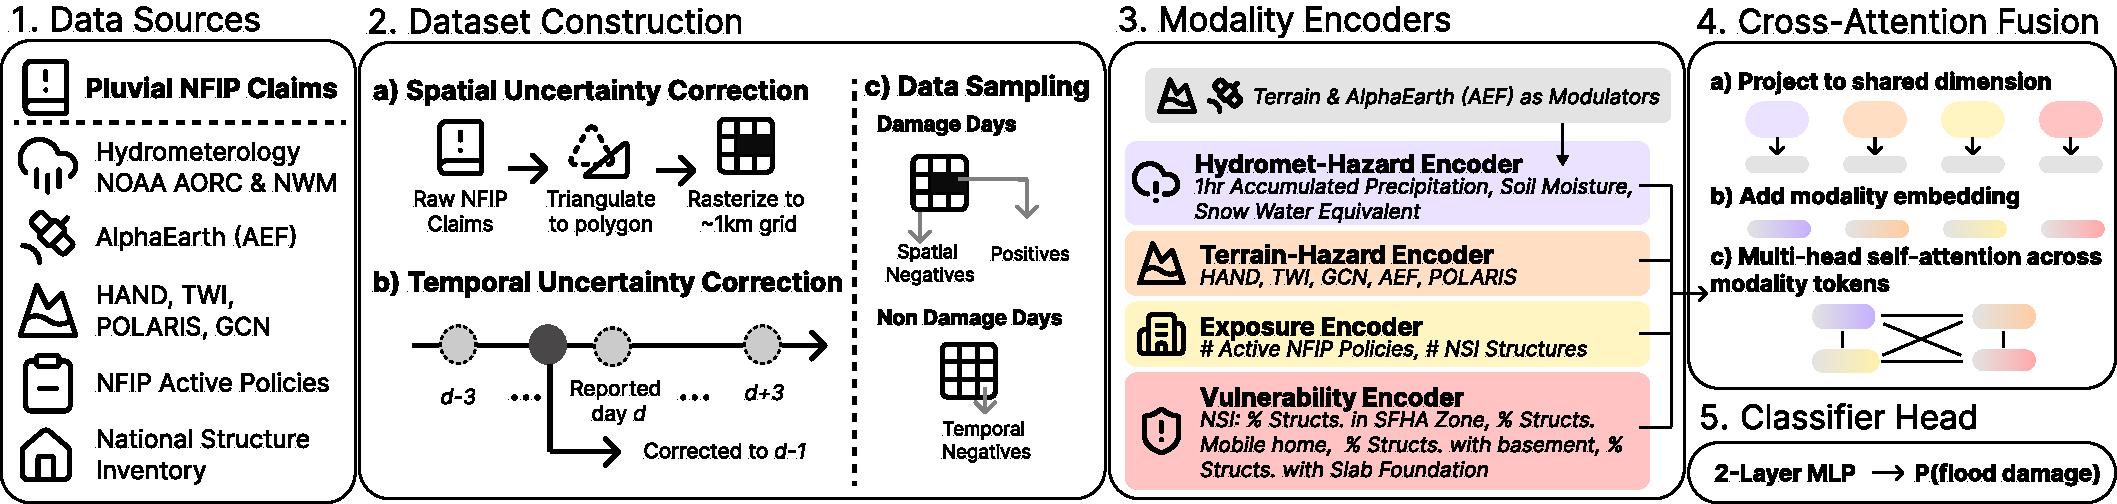
\includegraphics[width=\textwidth]{figs/Workflow.pdf}
    \caption{\textbf{DELUGE architecture.} DELUGE is a multimodal CNN-based model that integrates various data modalities, including meteorological, terrain-hazard, vulnerability, and exposure features, to predict pluvial flood damage at a daily and $\sim$1km resolution across the CONUS. The model consists of separate CNN branches for each modality, which are then fused together to produce the final damage prediction.}
    \label{fig:deluge_architecture}
\end{figure*}
Pluvial flooding are localized events with dynamics that are highly dependent on local conditions, such as topography, land use, and drainage infrastructure. 
%
Past authors have identified the scale at which these flooding occurs and we select a approximately $8\times8$km grid cell as the spatial unit for our model, which is consistent with the spatial scale of pluvial flooding and associated hydrological process identified in the literature \cite{cristiano_spatial_2017}.
%
To capture these dynamics, we propose a multimodal CNN-based model, DELUGE, that leverages the local induction bias of CNNs to effectively model the spatial dependencies in pluvial flood damage prediction.
